%%%%%%%%%%%%%%%%%%%%%%%%%%%%%%%%%%%%
% Header                           %
%%%%%%%%%%%%%%%%%%%%%%%%%%%%%%%%%%%%
% 
% Revisions: 2017-04-10 Martin R�del <martin.raedel@dlr.de>
%                       Initial draft
%               
% Contact:   Martin R�del,  martin.raedel@dlr.de
%            DLR Composite Structures and Adaptive Systems
%          
%                                 __/|__
%                                /_/_/_/  
%            www.dlr.de/fa/en      |/ DLR
% 
%%%%%%%%%%%%%%%%%%%%%%%%%%%%%%%%%%%%
% Content                          %
%%%%%%%%%%%%%%%%%%%%%%%%%%%%%%%%%%%%

\levelstay{Visualize nodesets}

To visualize the nodesets from a \marktool{\exodusname} mesh or \marktool{\toolname} results file in \marktool{\paraviewname} perform the following steps

\begin{enumerate}[noitemsep]
\item From the menu bar: \label{itm:Use_ParaView_Visualize_NoseSet_Step1}
  \begin{itemize}[noitemsep]
  \item Click File
  \item Click Open
  \item Select the .g/.e-\marktool{\toolname} input or output file
  \end{itemize}
  or click 
\includegraphics[width=\iconsize]{Figures/Icons/pqOpen32} in the Main Controls toolbar
\item In the newly opened \textit{Properties} tab:
  \begin{itemize}[noitemsep]
  \item Click the gear symbol 
\includegraphics[width=\iconsize]{Figures/Icons/pqAdvanced26} next to the \textit{Search} line
  \item \textit{Sets} and \textit{Maps} tables become available for selection
  \item Select the nodesets to display
  \item Unselect all Blocks
  \item Click \textit{Apply}
  \end{itemize}
\item Create a \textit{Glyph} based on the current model as described in \autoref{sec:ParaView_Damage_Plots_on_Nodes_as_Spheres} (without the result data stuff of course)
\item Repeat step \ref{itm:Use_ParaView_Visualize_NoseSet_Step1}
\item In the newly opened \textit{Properties} tab:
  \begin{itemize}[noitemsep]
  \item Select all Blocks
  \item Set the \textit{Opacity} to 0.4
  \item Click \textit{Apply}
  \end{itemize}
\end{enumerate}

Similarly, the nodesets in the peridynamic collocation point translation can be visualized. The following figure shows the base \marktool{\exodusname} finite element mesh in gray. Superimposed with the finite element mesh are the nodes of a finite element nodeset (blue) and the nodeset in the peridynamic translation (green).

\begin{figure}[htbp]
\centering
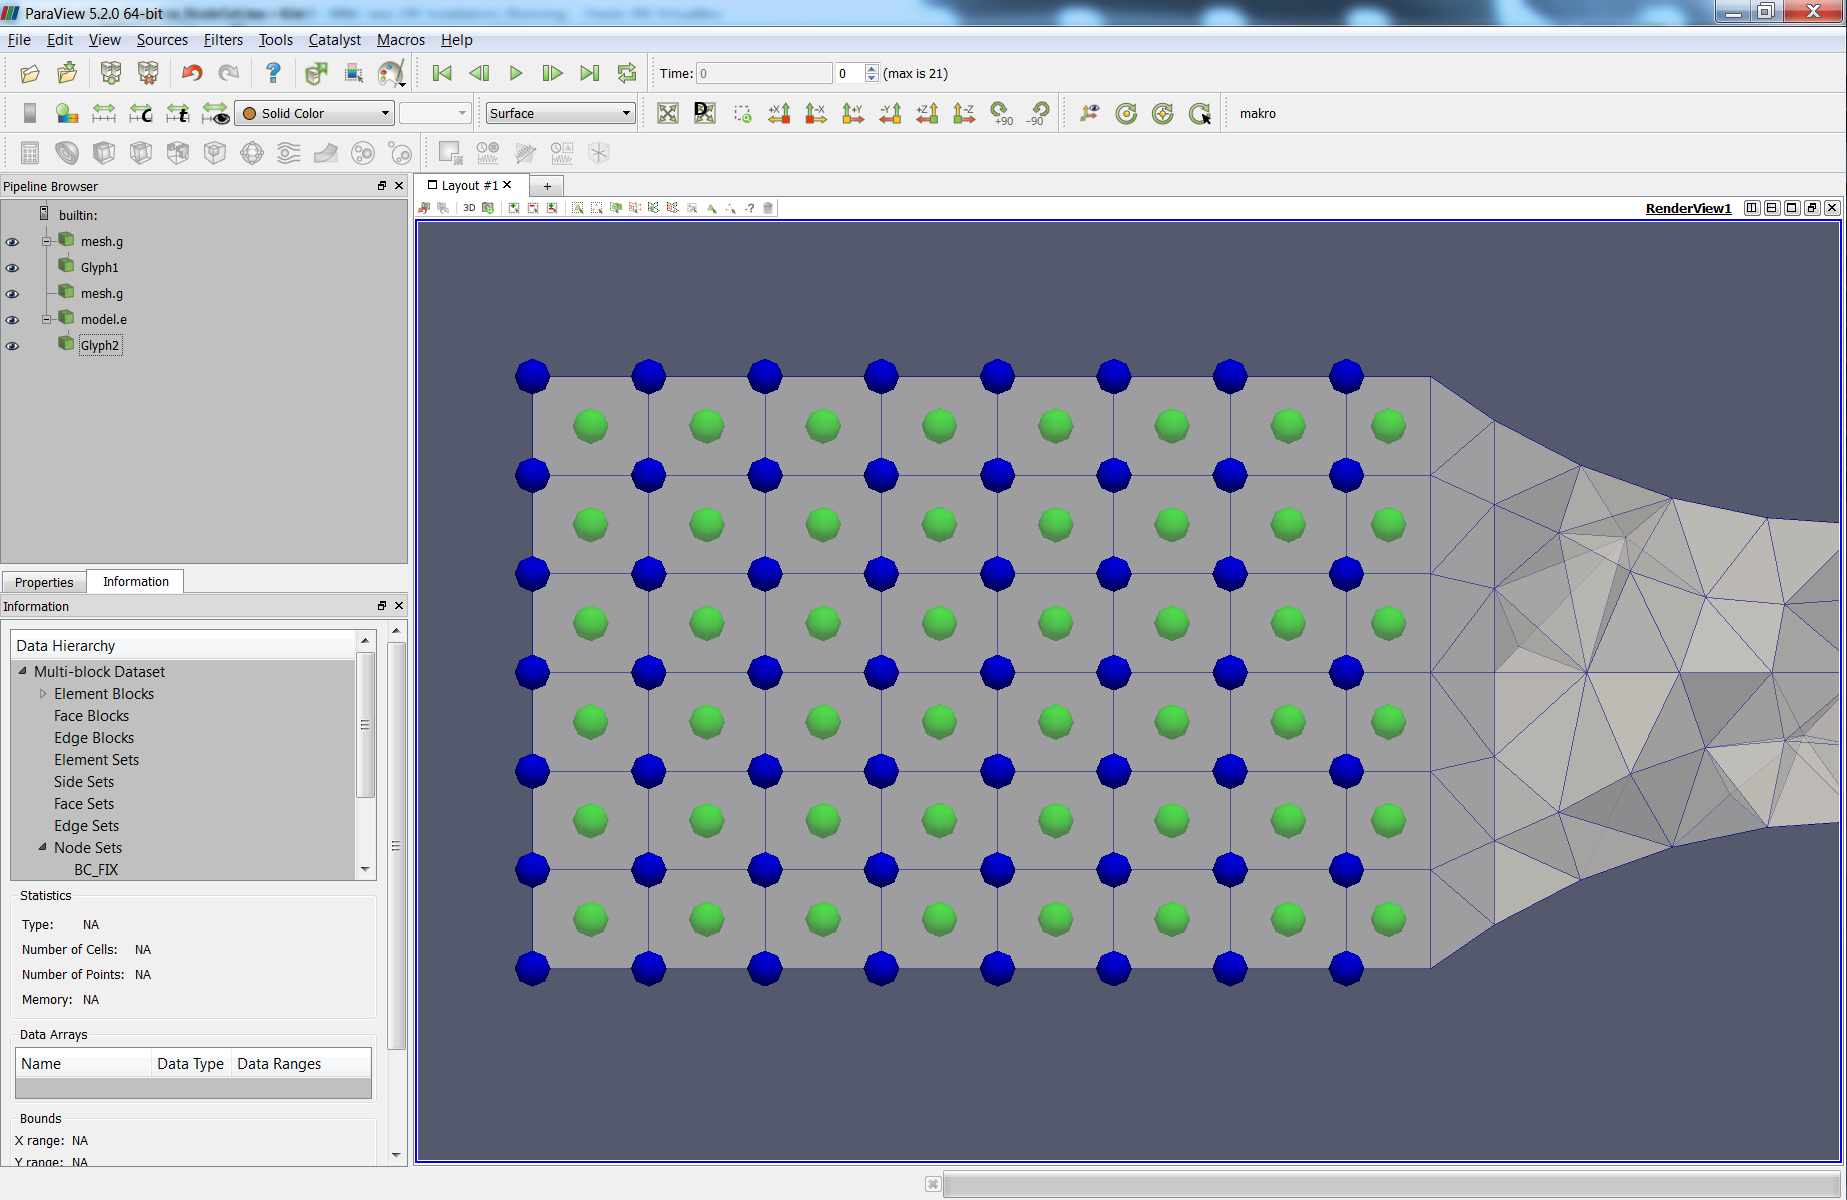
\includegraphics[width=\paraviewscreenshotwidthfac\linewidth]{Figures/Screenshots/ParaView_Visualize_NodeSets}
\caption{Visualization of base finite element mesh (gray), finite element nodeset (blue) and nodeset after transformation to peridynamic collocation points (green)}
\label{fig:Use_ParaView_Visualize_NoseSets}
\end{figure}

\FloatBarrier